% -----------------------------------------------------------------------------
\section{Purpose}
% -----------------------------------------------------------------------------
% Synthetic biology aims to apply engineering principles such as standardization, modularity, and design abstraction to molecular biology.  However, synthetic biology still faces substantial challenges, including long development times, high rates of failure, and poor reproducibility. 

% The Synthetic Biology Open Language is intended to help synthetic biologists collaborate by allowing them to exchange designs in a standardized data format.  In addition, the SBOL data model systematically describes the essential details of a design that are needed for researchers to reproduce each other's designs in the laboratory.  The purpose of the Synthetic Biology Open Language is to aid collaboration between researchers, improve scientific reproducibility, and to speed the research and development of technologies based on synthetic biology.

Synthetic biology builds upon the techniques and successes of genetics, molecular biology, and metabolic engineering by applying engineering principles to the design of biological systems. These principles include standardization, modularity, and design abstraction. The field still faces substantial challenges, including long development times, high rates of failure, and poor reproducibility. A common factor of these challenges is the exchange of information about designed systems between laboratories. 
When designing a synthetic system, synthetic biologists need to exchange information about multiple types of molecules and their expected behavior in the design.
Furthermore, there are often multiple degrees of separation between a specified nucleic acid sequence (e.g., a sequence that encodes an enzyme or transcription factor) and the molecular interactions that a designer intends to result from said sequence (e.g., chemical modification of metabolites or regulation of gene expression), yet these different perspectives need to be connected together in the engineering of biological systems.

The \emph{Synthetic Biology Open Language} (SBOL) has been developed as a standard to support the specification and exchange of biological design information in synthetic biology, filling a need not satisfied by other pre-existing standards.
Previous nucleic acid sequence description formats lack key capabilities. For example,  simple sequence encoding formats such as FASTA encode almost nothing about design rationale. More sophisticated formats such as GenBank and Swiss-Prot support a flat annotation of sequence features that is well suited to the  description of natural systems, but is unable to represent the multi-layered design structure common to engineered systems.
\ref{f:sequence} shows the relationship of selected prior sequence description formats to SBOL 1.x and SBOL 2.x.
Modeling languages, such as the Systems Biology Markup Language (SBML) ~\cite{SBML} can be used represent biological processes, but are not sufficient to represent the associated nucleotide or amino acid sequences.  %Goksel: Commented this sentence: Kinetic information might be present in SBML~\cite{SBML} or mass conservation laws in other systems such as the COBRA Toolbox~\cite{COBRA}. 
Synthetic biology needs a structured standard that defines how to represent relevant molecules and their functional roles within a designed system, standardized rules on how such information is encoded in a file format, and software libraries to enable the exchange of such data between participating laboratories and as part of the publication process. 
%Goksel: Updated the sentence as above:Systems Biology Markup Language (SBML) represents reactions, pathways, and models, but does not typically represent the associated sequences.

To help address these challenges, SBOL introduces a standardized format for the electronic exchange of information on the structural and functional aspects of biological designs. 
The standard has been designed to support the explicit and unambiguous description of biological designs by means of a well defined data model. 
The standard further describes the rules and best practices on how to use this data model and populate it with relevant design details. 
SBOL uses existing Semantic Web practices and resources, such as \emph{Uniform Resource Identifiers} (\sbol{URI}s) and ontologies, to unambiguously identify and define genetic design elements.
%Anil: I think we need to say just a bit more here about how we support extensions to the core data model using annotations. I think the sentences removed below were hinting at that. 
%Goksel: Replaced thi sentence with the one above:Because the standard itself can represent information from other sources for sequence representations, reaction information and ontologies to represent biological design information, the standard uses modern information exchange techniques such as \emph{Universal Resource Identifiers} (URIs). This permits the reuse of existing information without the need to repeat it, thus avoiding both redundancy and likely future information decay within shared files. 
%Goksel: Removed this sentence: The ultimate utility of URIs in the SBOL standard is the ability to support flexible annotation with appropriate metadata while associating an authority with that annotation. 
The definition of the data model and associated format, the rules on the addition of data within the format and the representation of this in electronic data files are intended to make the SBOL standard a useful means of promoting global data exchange between laboratories and between software programs.


This document details version 2.3 of SBOL that builds upon the previous version 2.2. In particular, SBOL 2.3 includes means of succinctly representing sequence modifications (such as insertion, deletion, and replacement), an extension to support organization and attachment of experimental data derived from designs,
and an extension for describing numerical parameters of design elements. The new version also includes typing of activities, unambiguous locations for sequences with multiple encodings, refinement of a number of validation rules, improved figures and examples, and clarification on a number of issues related to ontology terms. 


Version 2.2 of SBOL in turn builds upon SBOL version 2.1. SBOL 2.2 included improved description and validation rules for genetic design provenance, an extension to support combinatorial genetic designs, a new class to add non-SBOL data as attachments, a new class for genetic design implementations, and a description of a methodology to describe the entire design-build-test-learn cycle within the SBOL data model.

Version 2.1 included improved rules for what constitutes a valid SBOL document, new role fields to simplify the expression of sequence features and how components are used in context, and new best practices descriptions to improve the exchange of basic sequence topology information and the description of genetic design provenance.

SBOL 2.x builds upon SBOL 1.1, which focused on representing the structural aspects of genetic designs. Users of the standard were able to exchange information on DNA designs, but they could not represent molecules other than DNA or the functional aspects of designs beyond DNA sequence features. The SBOL 2 data model defined in this specification extends the version 1.1 data model to provide for the most pressing data exchange needs identified by the SBOL community. In particular, the extended data model can:
\begin{itemize}

\item Represent non-DNA structural components of a biological design, including RNA, proteins, small molecules and other physical components.

\item Describe the behavioral aspects of a biological design, such as the intended or expected molecular interactions, and link to mathematical models written in other standards

\item Associate structure and function so that a single design can be understood in terms of its structure, behavior, or both.

\item Support rich annotation of biological designs, so that classes of design data that are not explicitly covered by this specification can be safely exchanged

\end{itemize}
Taken together, these extensions enable SBOL to support the description and exchange of hierarchical, modular representations of both the intended structure and function of designed biological systems.

\begin{figure}[htbp]
\centering
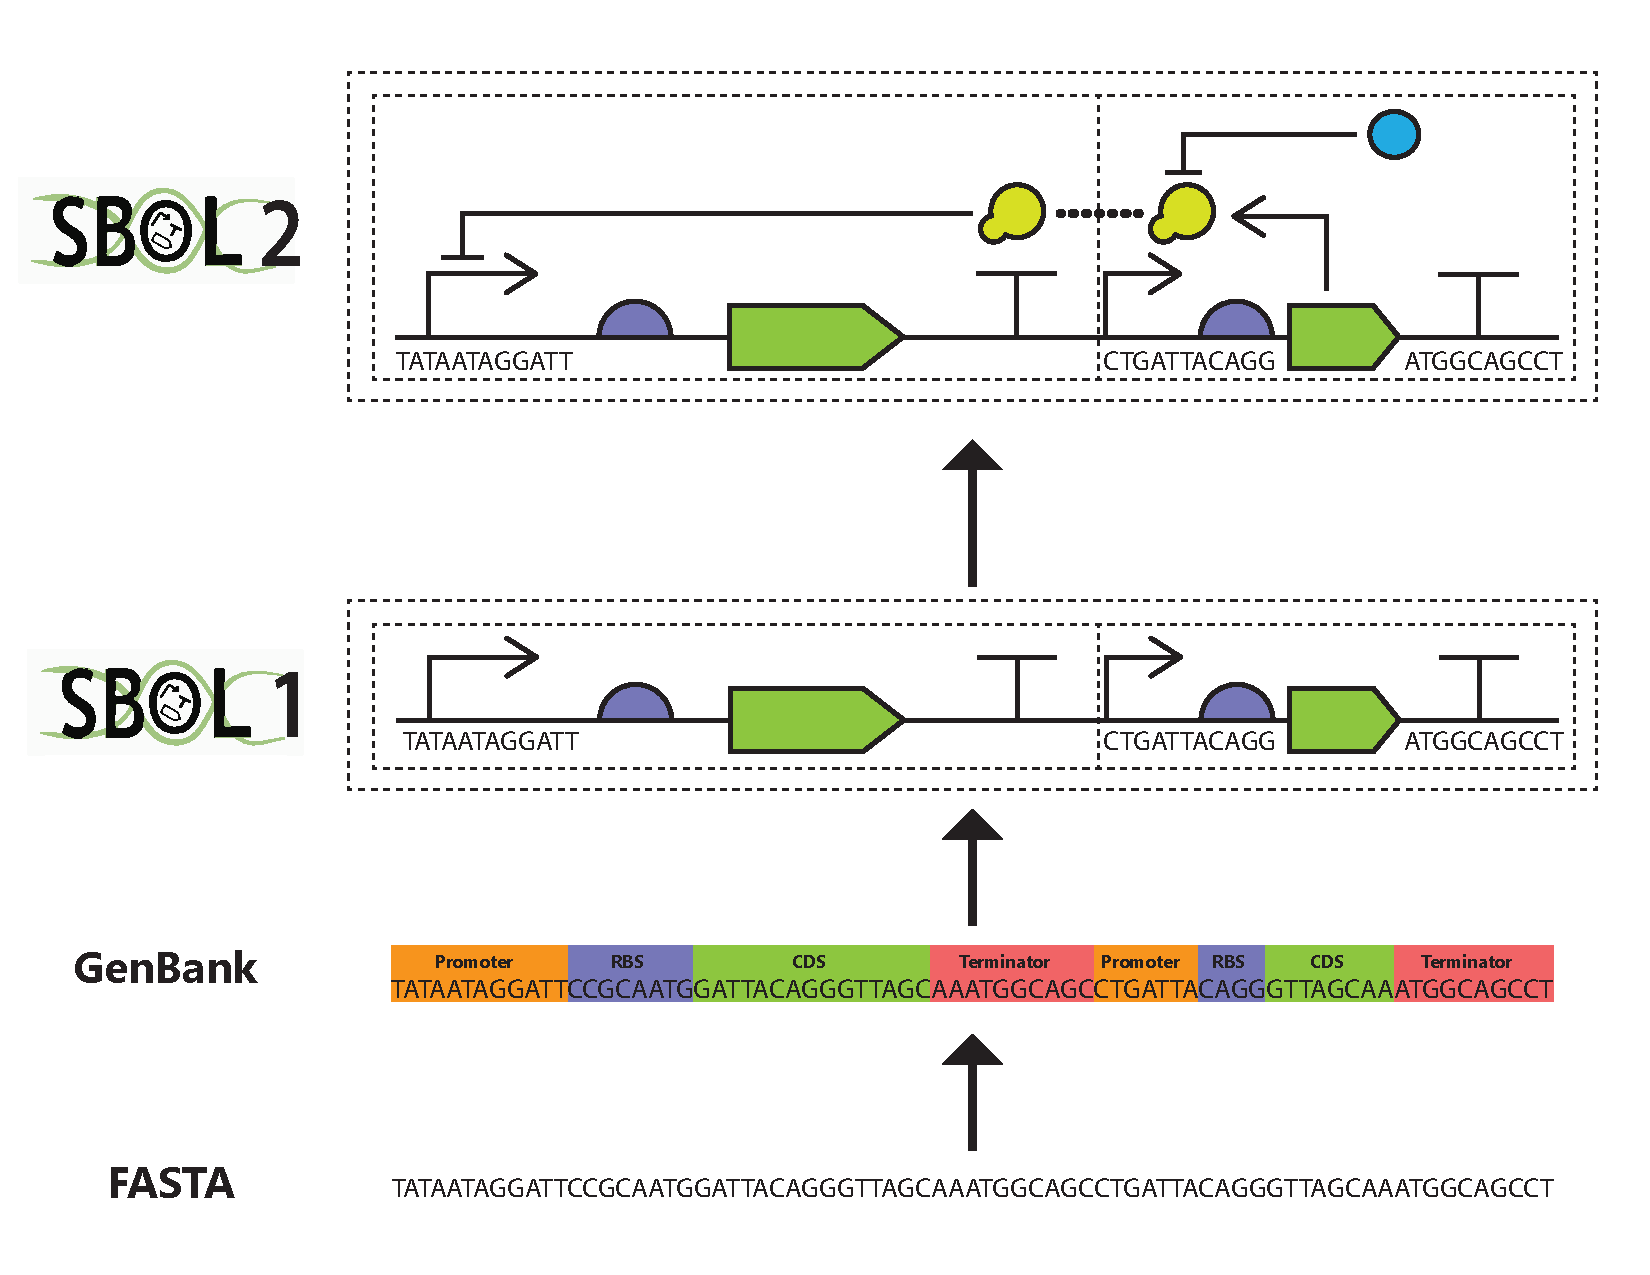
\includegraphics[width=\textwidth]{images/standard-evolution.pdf}
\caption{SBOL 2 extends prior sequence description formats to represent both the structure and function of a genetic design in a modular, hierarchical manner.}
\label{f:sequence}
\end{figure}


While the ultimate goal of SBOL is to describe synthetic biological designs such that they can be reproduced in the lab with a high degree of fidelity, SBOL 2 does not yet provide a complete catalog of the different classes of data that are necessary to achieve this goal. 
For example, SBOL 2 does not yet include data on environmental and host context, or details on how the performance of a design is measured. 
To enable progress towards capturing these types of data, SBOL 2 provides an annotation mechanism that allows SBOL to be easily extended (see \ref{sec:Annotations}). Three scenarios are envisaged for extending SBOL:

\begin{itemize}
\item Critical data related to the reproducibility of designs. These include  what growth media was used, what temperature the organisms were grown at, or where the recombinant DNA was integrated into the host genome or a plasmid.
\item Tool specific data. These could include tool settings specific to the design that is being loaded, such as which windows are to be opened or which settings are to be initialized. Tool makers could also include encrypted proprietary information related to a company or client in an extension. 
\item Data that are non-essential for  reproducibility but are nevertheless useful to many users. There are many cases where specific communities of users require data that cannot be explicitly represented using the SBOL data model. These include data on visualization, evolutionary stability, or other .
\end{itemize}

The extension mechanism is therefore a critical part of SBOL 2 and will allow others in the community to incorporate their own custom data into SBOL files and contribute to community efforts to expand the scope of SBOL.

% To address the need for functional descriptions in SBOL, the proposed data model adds new classes to provide a firm basis for functional representation in SBOL without going so far as to create a new standard for mathematically modeling biology, as there already exist several established languages for doing so, from the SBML to CellML~\cite{CellML} and even MATLAB~\cite{matlab}. Rather, these classes enable users of SBOL to group components that function together, describe the basic qualitative interactions between these components, and document references to standard mathematical models that are external to SBOL and that provide more detailed descriptions of component function. In other words, a module definition gathers together a set of component instantiations, a set of interactions between these component instantiations, and a set of references to external models that are expected to be consistent with the module's interactions.

The SBOL 2 specifications also add a number of measures to simplify adoption and validation of compatibility with the standard.
First, unlike the SBOL 1.1 specification, the SBOL 2 specification explicitly incorporates the primary serialization format for its data model to better show how the standard can be used. Second, the specification includes a set of validation rules for determining the compatibility of a document with SBOL 2, most of which are machine-verifiable. Finally, the specification includes a set of recommended best practices that can allow software tools to take best advantage of the standard and effectively exchange data.

In addition, care has been taken to ensure that all SBOL 2.x specifications are backwards-compatible with previous versions.
First, every SBOL 2.x file is also a valid SBOL 2.y file where y is greater than or equal to x.
Second, while the changes made in SBOL 2 do mean that an SBOL 1.x file is not a valid SBOL 2.x file, there does exist a direct mapping from the SBOL 1.x data model to the SBOL 2 data model, making it possible to automatically convert any SBOL 1.x file to an SBOL 2 file.
% Goksel - Removed this sentence:Therefore, SBOL 2.0 supersedes SBOL 1.1, and developers are encouraged to use it for all new software efforts.  
Since SBOL 2 can encode all data previously encoded in SBOL 1.1, developers are encouraged to upgrade their SBOL 1.1 compliant software tools to use SBOL 2 software libraries. 

Lastly, the SBOL standard has been developed in collaboration between both ``wet'' bench scientists and ``dry'' scientific modelers and software developers that are active within the synthetic biology community. 
As before with SBOL version 1.1, this open community has met to discuss and agree upon the data exchange needs that each version of the SBOL 2.x standard is intended to address. 
These discussions have informed the efforts of  developers within the community to produce a SBOL 2 specification after several rounds of proposal and revision. This specification has been evaluated by the community for its ability to represent a wide range of synthetic biology designs and share these designs between different laboratories. 
This specification has also informed the development of software libraries that implement the standard, and software tools that employ the standard by means of these libraries, thereby providing further testing of SBOL 2. 
The publication of this specification is intended to make these capabilities more widely accessible to potential developers and users in the synthetic biology community and beyond.
